
%% bare_conf.tex
%% V1.4
%% 2012/12/27
%% by Michael Shell
%% See:
%% http://www.michaelshell.org/
%% for current contact information.
%%
%% This is a skeleton file demonstrating the use of IEEEtran.cls
%% (requires IEEEtran.cls version 1.8 or later) with an IEEE conference paper.
%%
%% Support sites:
%% http://www.michaelshell.org/tex/ieeetran/
%% http://www.ctan.org/tex-archive/macros/latex/contrib/IEEEtran/
%% and
%% http://www.ieee.org/

%%*************************************************************************
%% Legal Notice:
%% This code is offered as-is without any warranty either expressed or
%% implied; without even the implied warranty of MERCHANTABILITY or
%% FITNESS FOR A PARTICULAR PURPOSE! 
%% User assumes all risk.
%% In no event shall IEEE or any contributor to this code be liable for
%% any damages or losses, including, but not limited to, incidental,
%% consequential, or any other damages, resulting from the use or misuse
%% of any information contained here.
%%
%% All comments are the opinions of their respective authors and are not
%% necessarily endorsed by the IEEE.
%%
%% This work is distributed under the LaTeX Project Public License (LPPL)
%% ( http://www.latex-project.org/ ) version 1.3, and may be freely used,
%% distributed and modified. A copy of the LPPL, version 1.3, is included
%% in the base LaTeX documentation of all distributions of LaTeX released
%% 2003/12/01 or later.
%% Retain all contribution notices and credits.
%% ** Modified files should be clearly indicated as such, including  **
%% ** renaming them and changing author support contact information. **
%%
%% File list of work: IEEEtran.cls, IEEEtran_HOWTO.pdf, bare_adv.tex,
%%                    bare_conf.tex, bare_jrnl.tex, bare_jrnl_compsoc.tex,
%%                    bare_jrnl_transmag.tex
%%*************************************************************************

% *** Authors should verify (and, if needed, correct) their LaTeX system  ***
% *** with the testflow diagnostic prior to trusting their LaTeX platform ***
% *** with production work. IEEE's font choices can trigger bugs that do  ***
% *** not appear when using other class files.                            ***
% The testflow support page is at:
% http://www.michaelshell.org/tex/testflow/



% Note that the a4paper option is mainly intended so that authors in
% countries using A4 can easily print to A4 and see how their papers will
% look in print - the typesetting of the document will not typically be
% affected with changes in paper size (but the bottom and side margins will).
% Use the testflow package mentioned above to verify correct handling of
% both paper sizes by the user's LaTeX system.
%
% Also note that the "draftcls" or "draftclsnofoot", not "draft", option
% should be used if it is desired that the figures are to be displayed in
% draft mode.
%
\documentclass[conference]{IEEEtran}
% Add the compsoc option for Computer Society conferences.
%
% If IEEEtran.cls has not been installed into the LaTeX system files,
% manually specify the path to it like:
% \documentclass[conference]{../sty/IEEEtran}





% Some very useful LaTeX packages include:
% (uncomment the ones you want to load)


% *** MISC UTILITY PACKAGES ***
%
%\usepackage{ifpdf}
% Heiko Oberdiek's ifpdf.sty is very useful if you need conditional
% compilation based on whether the output is pdf or dvi.
% usage:
% \ifpdf
%   % pdf code
% \else
%   % dvi code
% \fi
% The latest version of ifpdf.sty can be obtained from:
% http://www.ctan.org/tex-archive/macros/latex/contrib/oberdiek/
% Also, note that IEEEtran.cls V1.7 and later provides a builtin
% \ifCLASSINFOpdf conditional that works the same way.
% When switching from latex to pdflatex and vice-versa, the compiler may
% have to be run twice to clear warning/error messages.

\usepackage{amsmath}
\usepackage{amsfonts}
\usepackage{amssymb}

\usepackage{listings}
\usepackage{graphicx}
\graphicspath{{images/}}

\usepackage{caption}
\usepackage{subcaption}

\usepackage{multirow}


% *** CITATION PACKAGES ***
%
%\usepackage{cite}
% cite.sty was written by Donald Arseneau
% V1.6 and later of IEEEtran pre-defines the format of the cite.sty package
% \cite{} output to follow that of IEEE. Loading the cite package will
% result in citation numbers being automatically sorted and properly
% "compressed/ranged". e.g., [1], [9], [2], [7], [5], [6] without using
% cite.sty will become [1], [2], [5]--[7], [9] using cite.sty. cite.sty's
% \cite will automatically add leading space, if needed. Use cite.sty's
% noadjust option (cite.sty V3.8 and later) if you want to turn this off
% such as if a citation ever needs to be enclosed in parenthesis.
% cite.sty is already installed on most LaTeX systems. Be sure and use
% version 4.0 (2003-05-27) and later if using hyperref.sty. cite.sty does
% not currently provide for hyperlinked citations.
% The latest version can be obtained at:
% http://www.ctan.org/tex-archive/macros/latex/contrib/cite/
% The documentation is contained in the cite.sty file itself.

\usepackage[
backend=biber,
style=numeric,
sorting=nty,
]{biblatex}
\addbibresource{literature.bib}




% *** GRAPHICS RELATED PACKAGES ***
%
\ifCLASSINFOpdf
  % \usepackage[pdftex]{graphicx}
  % declare the path(s) where your graphic files are
  % \graphicspath{{../pdf/}{../jpeg/}}
  % and their extensions so you won't have to specify these with
  % every instance of \includegraphics
  % \DeclareGraphicsExtensions{.pdf,.jpeg,.png}
\else
  % or other class option (dvipsone, dvipdf, if not using dvips). graphicx
  % will default to the driver specified in the system graphics.cfg if no
  % driver is specified.
  % \usepackage[dvips]{graphicx}
  % declare the path(s) where your graphic files are
  % \graphicspath{{../eps/}}
  % and their extensions so you won't have to specify these with
  % every instance of \includegraphics
  % \DeclareGraphicsExtensions{.eps}
\fi
% graphicx was written by David Carlisle and Sebastian Rahtz. It is
% required if you want graphics, photos, etc. graphicx.sty is already
% installed on most LaTeX systems. The latest version and documentation
% can be obtained at: 
% http://www.ctan.org/tex-archive/macros/latex/required/graphics/
% Another good source of documentation is "Using Imported Graphics in
% LaTeX2e" by Keith Reckdahl which can be found at:
% http://www.ctan.org/tex-archive/info/epslatex/
%
% latex, and pdflatex in dvi mode, support graphics in encapsulated
% postscript (.eps) format. pdflatex in pdf mode supports graphics
% in .pdf, .jpeg, .png and .mps (metapost) formats. Users should ensure
% that all non-photo figures use a vector format (.eps, .pdf, .mps) and
% not a bitmapped formats (.jpeg, .png). IEEE frowns on bitmapped formats
% which can result in "jaggedy"/blurry rendering of lines and letters as
% well as large increases in file sizes.
%
% You can find documentation about the pdfTeX application at:
% http://www.tug.org/applications/pdftex





% *** MATH PACKAGES ***
%
%\usepackage[cmex10]{amsmath}
% A popular package from the American Mathematical Society that provides
% many useful and powerful commands for dealing with mathematics. If using
% it, be sure to load this package with the cmex10 option to ensure that
% only type 1 fonts will utilized at all point sizes. Without this option,
% it is possible that some math symbols, particularly those within
% footnotes, will be rendered in bitmap form which will result in a
% document that can not be IEEE Xplore compliant!
%
% Also, note that the amsmath package sets \interdisplaylinepenalty to 10000
% thus preventing page breaks from occurring within multiline equations. Use:
%\interdisplaylinepenalty=2500
% after loading amsmath to restore such page breaks as IEEEtran.cls normally
% does. amsmath.sty is already installed on most LaTeX systems. The latest
% version and documentation can be obtained at:
% http://www.ctan.org/tex-archive/macros/latex/required/amslatex/math/





% *** SPECIALIZED LIST PACKAGES ***
%
%\usepackage{algorithmic}
% algorithmic.sty was written by Peter Williams and Rogerio Brito.
% This package provides an algorithmic environment fo describing algorithms.
% You can use the algorithmic environment in-text or within a figure
% environment to provide for a floating algorithm. Do NOT use the algorithm
% floating environment provided by algorithm.sty (by the same authors) or
% algorithm2e.sty (by Christophe Fiorio) as IEEE does not use dedicated
% algorithm float types and packages that provide these will not provide
% correct IEEE style captions. The latest version and documentation of
% algorithmic.sty can be obtained at:
% http://www.ctan.org/tex-archive/macros/latex/contrib/algorithms/
% There is also a support site at:
% http://algorithms.berlios.de/index.html
% Also of interest may be the (relatively newer and more customizable)
% algorithmicx.sty package by Szasz Janos:
% http://www.ctan.org/tex-archive/macros/latex/contrib/algorithmicx/




% *** ALIGNMENT PACKAGES ***
%
%\usepackage{array}
% Frank Mittelbach's and David Carlisle's array.sty patches and improves
% the standard LaTeX2e array and tabular environments to provide better
% appearance and additional user controls. As the default LaTeX2e table
% generation code is lacking to the point of almost being broken with
% respect to the quality of the end results, all users are strongly
% advised to use an enhanced (at the very least that provided by array.sty)
% set of table tools. array.sty is already installed on most systems. The
% latest version and documentation can be obtained at:
% http://www.ctan.org/tex-archive/macros/latex/required/tools/


% IEEEtran contains the IEEEeqnarray family of commands that can be used to
% generate multiline equations as well as matrices, tables, etc., of high
% quality.




% *** SUBFIGURE PACKAGES ***
%\ifCLASSOPTIONcompsoc
%  \usepackage[caption=false,font=normalsize,labelfont=sf,textfont=sf]{subfig}
%\else
%  \usepackage[caption=false,font=footnotesize]{subfig}
%\fi
% subfig.sty, written by Steven Douglas Cochran, is the modern replacement
% for subfigure.sty, the latter of which is no longer maintained and is
% incompatible with some LaTeX packages including fixltx2e. However,
% subfig.sty requires and automatically loads Axel Sommerfeldt's caption.sty
% which will override IEEEtran.cls' handling of captions and this will result
% in non-IEEE style figure/table captions. To prevent this problem, be sure
% and invoke subfig.sty's "caption=false" package option (available since
% subfig.sty version 1.3, 2005/06/28) as this is will preserve IEEEtran.cls
% handling of captions.
% Note that the Computer Society format requires a larger sans serif font
% than the serif footnote size font used in traditional IEEE formatting
% and thus the need to invoke different subfig.sty package options depending
% on whether compsoc mode has been enabled.
%
% The latest version and documentation of subfig.sty can be obtained at:
% http://www.ctan.org/tex-archive/macros/latex/contrib/subfig/




% *** FLOAT PACKAGES ***
%
%\usepackage{fixltx2e}
% fixltx2e, the successor to the earlier fix2col.sty, was written by
% Frank Mittelbach and David Carlisle. This package corrects a few problems
% in the LaTeX2e kernel, the most notable of which is that in current
% LaTeX2e releases, the ordering of single and double column floats is not
% guaranteed to be preserved. Thus, an unpatched LaTeX2e can allow a
% single column figure to be placed prior to an earlier double column
% figure. The latest version and documentation can be found at:
% http://www.ctan.org/tex-archive/macros/latex/base/


%\usepackage{stfloats}
% stfloats.sty was written by Sigitas Tolusis. This package gives LaTeX2e
% the ability to do double column floats at the bottom of the page as well
% as the top. (e.g., "\begin{figure*}[!b]" is not normally possible in
% LaTeX2e). It also provides a command:
%\fnbelowfloat
% to enable the placement of footnotes below bottom floats (the standard
% LaTeX2e kernel puts them above bottom floats). This is an invasive package
% which rewrites many portions of the LaTeX2e float routines. It may not work
% with other packages that modify the LaTeX2e float routines. The latest
% version and documentation can be obtained at:
% http://www.ctan.org/tex-archive/macros/latex/contrib/sttools/
% Do not use the stfloats baselinefloat ability as IEEE does not allow
% \baselineskip to stretch. Authors submitting work to the IEEE should note
% that IEEE rarely uses double column equations and that authors should try
% to avoid such use. Do not be tempted to use the cuted.sty or midfloat.sty
% packages (also by Sigitas Tolusis) as IEEE does not format its papers in
% such ways.
% Do not attempt to use stfloats with fixltx2e as they are incompatible.
% Instead, use Morten Hogholm'a dblfloatfix which combines the features
% of both fixltx2e and stfloats:
%
% \usepackage{dblfloatfix}
% The latest version can be found at:
% http://www.ctan.org/tex-archive/macros/latex/contrib/dblfloatfix/




% *** PDF, URL AND HYPERLINK PACKAGES ***
%
%\usepackage{url}
% url.sty was written by Donald Arseneau. It provides better support for
% handling and breaking URLs. url.sty is already installed on most LaTeX
% systems. The latest version and documentation can be obtained at:
% http://www.ctan.org/tex-archive/macros/latex/contrib/url/
% Basically, \url{my_url_here}.




% *** Do not adjust lengths that control margins, column widths, etc. ***
% *** Do not use packages that alter fonts (such as pslatex).         ***
% There should be no need to do such things with IEEEtran.cls V1.6 and later.
% (Unless specifically asked to do so by the journal or conference you plan
% to submit to, of course. )


% correct bad hyphenation here
\hyphenation{op-tical net-works semi-conduc-tor}


\begin{document}
%
% paper title
% can use linebreaks \\ within to get better formatting as desired
% Do not put math or special symbols in the title.
\title{Time Series Forecasting Overview}


% author names and affiliations
% use a multiple column layout for up to three different
% affiliations
\author{\IEEEauthorblockN{Domen Mohorčič}
\IEEEauthorblockA{Faculty of Computer and\\Information Science\\
University of Ljubljana\\
Email: dm4492@student.uni-lj.si}
}

% conference papers do not typically use \thanks and this command
% is locked out in conference mode. If really needed, such as for
% the acknowledgment of grants, issue a \IEEEoverridecommandlockouts
% after \documentclass

% for over three affiliations, or if they all won't fit within the width
% of the page, use this alternative format:
% 
%\author{\IEEEauthorblockN{Michael Shell\IEEEauthorrefmark{1},
%Homer Simpson\IEEEauthorrefmark{2},
%James Kirk\IEEEauthorrefmark{3}, 
%Montgomery Scott\IEEEauthorrefmark{3} and
%Eldon Tyrell\IEEEauthorrefmark{4}}
%\IEEEauthorblockA{\IEEEauthorrefmark{1}School of Electrical and Computer Engineering\\
%Georgia Institute of Technology,
%Atlanta, Georgia 30332--0250\\ Email: see http://www.michaelshell.org/contact.html}
%\IEEEauthorblockA{\IEEEauthorrefmark{2}Twentieth Century Fox, Springfield, USA\\
%Email: homer@thesimpsons.com}
%\IEEEauthorblockA{\IEEEauthorrefmark{3}Starfleet Academy, San Francisco, California 96678-2391\\
%Telephone: (800) 555--1212, Fax: (888) 555--1212}
%\IEEEauthorblockA{\IEEEauthorrefmark{4}Tyrell Inc., 123 Replicant Street, Los Angeles, California 90210--4321}}

% use for special paper notices
%\IEEEspecialpapernotice{(Invited Paper)}




% make the title area
\maketitle

% As a general rule, do not put math, special symbols or citations
% in the abstract
\begin{abstract}
Time series is a special type of data, collected at even time intervals for longer periods of time. Time series forecasting is the task of predicting those sequences into the future. The task is important for commercial and environmental reasons, because with accurate predictions we can prepare for the forecasted scenario and either take its full advantage or mitigate it. A number of approaches have been proposed for time series forecasting. The earliest ones were simple linear autoregression models, but lately a lot of different approaches have been proposed: matrix factorization, transformers, deep, recurent, convolutional, and graph neural networks. We replicate the results from different papers, compare different models on the same dataset, and confirm that the current state-of-the-art model is indeed the best at time series forecasting.
\end{abstract}

% no keywords

% For peer review papers, you can put extra information on the cover
% page as needed:
% \ifCLASSOPTIONpeerreview
% \begin{center} \bfseries EDICS Category: 3-BBND \end{center}
% \fi
%
% For peerreview papers, this IEEEtran command inserts a page break and
% creates the second title. It will be ignored for other modes.
\IEEEpeerreviewmaketitle

\section{Introduction}

Time series is a sequence data, collected at even time intervals.
It is ordered and usually has multiple real-valued observations for each timestamp.
Time series forecasting (TSF) is a task of predicting the next values in such series.
It is important in the fields of climate modeling, medicine, commercial decision making, and finance.
With climate modeling \cite{mudelsee2019climate} we can predict and analyze the average temperature increase over time and forecast possible climate events that would have a huge impact on our way of living.
The most common climate forecasting is weather forecasting.
We use it every day to dress appropriately.
Financial firms use TSF to predict when and where markets will move.
With a good model they can make a lot of money by knowing when to buy and when to sell.
In medicine TSF can be used for seizure prediction \cite{elger1998siezure} and helping patients before they have one.
And in commercial decision making the TSF can be used to predict the sales of a specific item.
If the predicted sales go up, the company can prepare for it by having more stock to ensure they will not run out of specific item.

TSF task can be divided into categories based on two different criteria: forecast horizon and number of variables predicted.

The forecast horizon divides the problem into two categories: single- and multi-horizon forecasting.
In single-horizon forecasting the model predicts only one step at a time.
Multi-horizon forecasting tries to predict multiple steps into the future.
Even though single-horizon forecasting methods are more accurate than multi-horizon ones, multi-horizon forecasting is more valuable.
Decision makers use multi-horizon forecasting as it allows them to make better and more informed decisions as it gives more context and provides possible trends in the future.
A single-horizon method can be converted into a multi-horizon one with iteration, but will be less accurate than a direct multi-horizon method.
Because of all the advantages of multi-horizon over single-horizon forecasting, multi-horizon forecasting is the ultimate goal of TSF.

Number of variables predicted is the next criteria.
It divides TSF problem into two categories: univariate and multivariate.
Univariate TSF focuses on predicting one variable, while multivariate TSF tries to predict multiple variables at the same time.
The multivariate methods take into account multiple variables, but can also predict only one variable, if others are known ahead of time.
Multivariate methods are preferred, since we can get better predictions if we can learn the correlation between multiple variables.
Another problem here is the availability of variables.
If we predict only one variable but base our prediction on many, we need to have values for these variables in the future.
If those values do not exist at the time of prediction, a multivariate model that predicts all variables is used, but can be less accurate.
Univariate models have no such problems, as they base their next predictions automatically on previously forecasted values.

The aim of this report is to make an overview of the TSF in the last decade. In Chapter \ref{chap:models} we take a closer look at different models. In Chapter \ref{chap:data} we take a quick look at most popular TSF datasets and metrics and in Chapter \ref{chap:results} we test the models.
In this report we will focus on multi-horizon univariate forecasting models.

\section{Related work}
\label{chap:related}

The prediction of time series began in the previous century.
The first methods used were Autoregression (AR) and Moving Average (MA).
AR and MA models use linear combination of previous observations and depend on the domain expertise.
In 1968 Box, Jenkins, and MacGregor combined these two methods into Autoregressive Integrated Moving Average (ARIMA) model \cite{box1968arima}.
The Equation \ref{eq:arima} represents the ARIMA model, where $X_{t}$ is the prediction at time $t$, $\epsilon_{t}$ is the error at time $t$, and $\alpha$ and $\beta$ are just linear coefficients.
It can accurately forecast for short periods of time and tends to converge to a single value after long forecasting periods.
The ARIMA model is a univariate single-horizon method and will be used as a baseline.

\begin{equation}
    \label{eq:arima}
    X_{t} - \alpha _{1}X_{t-1} - \dots - \alpha _{p}X_{t-p} = \epsilon_{t} + \theta_{1}\epsilon_{t-1} + \dots + \theta_{q}\epsilon_{t-q}
\end{equation}

In the recent years a lot of different approaches have been tried.
In 2016 Yu, Rao, and Dhillon proposed the use of matrix factorization technique called Temporal Regularized Matrix Factorization (TRMF) in paper \cite{yu2016trmf}.
The method was developed with intentions to be highly scalable, and can also deal with highly noisy or missing data.
It builds on the idea to use graph regularization for matrix factorization (MF), but uses well-known time series models to describe temporal dependencies and as a regularization.
It was tested against other MF methods and performed significantly better.
It also proved to be very good for missing data imputation.

In year 2018 Lai et al. proposed a neural network called LSTNet in \cite{lai2018lstnet}.
The network is a combination of recurrent neural network (RNN) and a convolutional neural network (CNN).
It uses convolution to extract short-term patterns in the data.
Recurrent components capture periodic patterns, and the whole model incorporates auto-regressive model in parallel to keep the linear component.
The method was tested against other models on four different standard datasets and performed better than all of them.

The DeepAR model was designed and proposed by Salinas, Flunkert, and Gasthaus in 2019 in \cite{salinas2019deepar}.
It is a method for producing probabilistic forecasts, and it is an auto-regressive RNN.
It was build on the ideas from paper \cite{sutskever2014sequence}, posted in 2014, where authors Sutskever, Vinyals, and Le introduced a sequence to sequence RNN model for translation purposes.
DeepAR model uses inputs as well as last predictions to forecast values.
When compared to other models it performed better, but on some datasets yielded comparable results.

In 2017 a novel transformer approach was introduced by Vaswani et al. in \cite{vaswani2017attention}.
They proposed a model which relies on self-attention rather than a reference window and uses encoder-decoder structure to generate text.
In theory self-attention provides an infinite window length, meaning the model can always find relevant text it encountered somewhere before and generate text with relevant context.
In 2020 researchers Lim et al. in \cite{li2020enhancing} proposed a temporal fusion transformer, a model based on the original transformer, but for TSF purposes. They called it log-sparse transformer.
It uses recurrent layers for local processing and multi-head self-attention layers for long-term dependencies to create multi-horizon predictions.
The model performed better than all of its predecessors.

A year later, in 2021, Informer was introduced by Zhou et al. in \cite{zhou2021informer} as another upgrade to the original transformer, which had a few issues: quadratic time complexity, memory bottleneck for long inputs, and slow prediction times for long outputs.
Informer implemented probsparse self-attention to reduce learning time complexity from $O(n^{2})$ to $O(n logn)$.
It also has smaller feature map, which enabled faster calculation of predictions.
Informer performed better than other models both on univariate and multivariate predictions.

In 2020 researchers Wu et al. proposed a novel graph neural network (GNN) approach for TSF and presented it in \cite{wu2020connecting}.
GNN assumes that state of a node depends on the state of its neighbors, so a graph structure with predefined relationships between variables was required in models, known as spatial-temporal GNN.
Wu et al. proposed a MTGNN model where each node is a variable and the model learns connections and the graph structure by itself.
The model performed better than other GNN models for single-horizon forecasting and comparable for multi-horizon forecasting.

In 2020 researchers Oreshkin et al. presented a deep neural network (DNN) called N-Beats in \cite{oreshkin2020nbeats}.
It is unique in a way that it uses only fully connected layers and nothing else.
It consists of building blocks that output a forecast and a backcast to help future building blocks with forecasting.
The model was designed to be interpretable, so it uses periodic and small degree polynomial functions as mapping functions, which mimic seasonality and trend.
The model was compared to other M competition \cite{wikiMcomp} models and consistently performed better.

Liu et al. revisited convolutional neural networks (CNN) in late 2021 and proposed a new model, called SCINet, in \cite{liu2021scinet}.
SCINet model is a hierarchical model that captures temporal dependencies at multiple resolutions.
The model splits the data into even and odd and learns trends on them separately.
This procedure is repeated recursively, so the model learns from small and local to large and global trends.
The model is currently the state-of-the-art and preformed better at all standard TSF datasets.

\section{Models}
\label{chap:models}

In this section we will take a look at some of the above mentioned methods in detail. We will describe in detail the workings of TRMF, DeepAR, Informer, MTGNN, and SCINet.

\subsection{\textbf{TRMF}}

TRMF method is a MF model.
It was proposed to handle large number of observations through longer periods of time.
It was designed to handle climate data, where there are potentially thousands of sensors measuring every hour over a decade.
Some sensors can break, so the data can have missing values.
Normal models cannot deal with missing data, so some other preprocessing must be performed.

A natural way of modeling high dimensional data is in the form of a matrix, where rows are sensors and columns correspond to time points.
The MF method tries to factorize input matrix into two smaller matrices, $Y = FX$.
The TRMF model tries to minimize the expression in Equation \ref{eq:trfm}, where $\Omega$ is a set of observed entries at time $t$ and variable $i$ and $Y_{i,t}$ is the observation.
Matrices $X$ and $F$ represent time-varying variables and features for each time series respectively.
$\lambda$ represents regularization coefficient and $R$ represents regularization function.

\begin{equation}
\label{eq:trfm}
    \sum_{(i, t) \in \Omega} (Y_{i,t}-f_{i}^{T}x_{t})^{2}+\lambda_{f}R_{f}(F)+\lambda_{x}R_{x}(X)
\end{equation}

In standard MF squared Frobenius norm is used as a regularization.
It assumes no dependencies among variables, so it is not suitable.
Another technique is graph regularization for temporal dependencies, where we specify dependency pattern with a lag set $L$ such that all edges of distance $l \in L$ share the same weight $w_{l}$.
In such a graph nodes represent the observations.
The graph regularization is defined in Equation \ref{eq:trmf_graph}, where $G$ represents graph and $\mu$ represents regularization coefficient.

\begin{equation}
\label{eq:trmf_graph}
    R(X\mid G, \mu) = \frac{1}{2}\sum_{l\in L}\sum_{t;t>l}w_{l}(x_{t}-x_{t-l})^{2}+\frac{\mu}{2} \sum_{t}\|x_{t}\|^{2}
\end{equation}

It has few problems, since $w_{t} = 0$ would minimize the regularization.
Authors took the ideas from it and proposed to use a TSF model $M$ to describe dependencies.
Such model is described in Equation \ref{eq:trmf_model}, where $\Theta$ represents parameters of the model and $\epsilon_{t}$ are the residuals.

\begin{equation}
\label{eq:trmf_model}
    x_{t} = M_{\Theta}({x_{t-l}:l\in L})+\epsilon_{t}
\end{equation}

The new regularizer thus encourages the structure, introduced by $M$, and the resulting regularizing function is in Equation \ref{eq:trmf_reg}.
$T_{M} (X \mid \Theta)$ is the negative log likelihood of observing a particular value at time $t$ given model $M$ and its parameters $\Theta$.

\begin{equation}
\label{eq:trmf_reg}
    R_{x}(X) = T_{M}(X\mid \Theta) = -log P(x_{1}, \dots, x_{T} \mid \Theta)
\end{equation}

In Equation \ref{eq:trfm} the regularization term for $X$ is substituted with Equation \ref{eq:trmf_reg}.
We treat $\Theta$ as another set of variables, and the Equation \ref{eq:trfm} can be solved by an alternating minimization over $F$, $X$, and $\Theta$.
The forecasting is done by using model $M$ to predict future latent embedding of input and use $F$ to obtain forecasts. 

\subsection{\textbf{DeepAR}}

The DeepAR model is a RNN autoregression model that makes probabilistic forecasts.
The model is also a sequence-to-sequence model, meaning minimal feature engineering is required to capture the group behaviour.
It makes probabilistic forecasts based on Monte Carlo estimations that are consistent throughout time.
The model also has the ability to forecast time series that it has not seen during training, as it infers its predictions by learning from similar variables.

The goal of DeepAR is to model the conditional distribution $P(z_{i,t_{0}},\dots,z_{i, t_{T}} \mid z_{i,1},\dots,z_{i, t_{0}-1}, x_{i,1},\dots,x_{i, T})$, where $z_{i, t}$ are values of time series $i$ at time $t$ and $x_{i, t}$ are covariates.
The model distribution is given by a product of likelihood factors for each time $t$, given by the Equation \ref{eq:deepar_like}.
$h_{i, t}$ is the value of the network at time $t$, $\Theta$ represents model parameters, and $\theta$ is a function of the network input.

\begin{equation}
\label{eq:deepar_like}
    Q_{\Theta}(z_{i,t_{0}:T} \mid z_{i,1:t_{0}-1}, x_{i, 1:T}) = \Pi_{t=t_{0}}^{T}l(z_{i, t} \mid \theta(h_{i, t}, \Theta))
\end{equation}

The likelihood model $l$ determines the noise model of the data and should be chosen to match the statistical properties of the data.
DeepAR model predicts all parameters of $\theta$ for the next time point, so the noise model can change over time.
With Gaussian likelihood model, which is parametrized with mean $\mu$ and variance $\sigma^{2}$, the likelihood function becomes the probability density function of normal distribution.
The parameters of the model can be learned by maximizing the sum of the log-likelihood function.

The covariates $x_{i, t}$ can be item-dependent, time-dependent, or both.
They are used to provide additional information about the item or the time point to the model.
The covariates are standardized to have zero mean and unit variance.

\subsection{\textbf{Informer}}

\begin{figure}
    \centering
    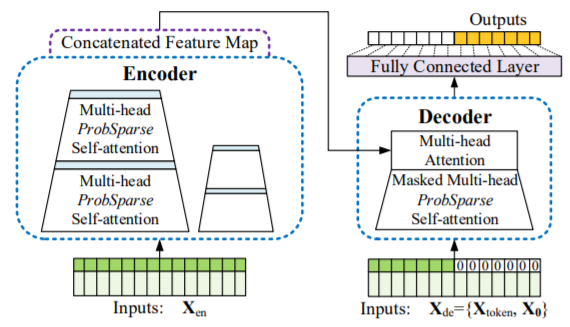
\includegraphics[width=0.48\textwidth]{informer.png}
    \caption{The architecture of the Informer model. The encoder learns feature representation while the decoder takes care of forecasting.}
    \label{fig:informer}
\end{figure}

The Informer model is a version of the transformer model, which was proposed for natural language processing tasks.
The architecture of the Informer model can be seen on Figure \ref{fig:informer}.
The model was designed to operate on long sequences, which is better for TSF problem, as we can forecast further in the future.
The transformer uses an encoder-decoder architecture and introduces self-attention for long sequence analysis, but is inefficient due to quadratic time complexity.
Some newer models proposed sparse and log-sparse self-attention, which solved time complexity problem.

The advantage of Informer is prob-sparse self-attention.
The original self-attention, proposed by transformer paper, is presented in Equation \ref{eq:trans}, where $Q$ is the query, $K$ is the key, $V$ is the value, and $d$ is the input dimension.
The query's attention is defined in Equation \ref{eq:query}, where the expression in the first sum represents the probability of key based on some query $p(k_{j}\mid q_{i})$.
The self-attention combines the values and makes outputs based on computing that probability.

\begin{equation}
\label{eq:trans}
    A(Q, K, V) = Softmax\left(\frac{QK^{t}}{\sqrt{d}}V\right)
\end{equation}

\begin{equation}
\label{eq:query}
    A(q_{i}, K, V) = \sum_{j}\frac{k(q_{i}, k_{j})}{\sum_{l}k(q_{i}, k_{l})}
\end{equation}

If $p(k_{j}\mid q_{i})$ approaches uniform distribution, the self-attention becomes redundant.
We can use Kullback-Lieber divergence to distinguish between distributions and find important queries.
The result is query's sparsity measurement, $M$.
The higher the value of $M$, the more important the query is.
The proposed prob-sparse self-attention is presented in Equation \ref{eq:probsparse}, where $\overline{Q}$ is a sparse matrix that contains only top queries under the sparsity measurement. 

\begin{equation}
\label{eq:probsparse}
    A(Q, K, V) = Softmax\left(\frac{\overline{Q}K^{t}}{\sqrt{d}}V\right)
\end{equation}

As a consequence of prob-sparse self-attention, the feature map has redundant values of $V$.
Authors use distilling, which suppresses redundant values and makes a more focused feature map.

The decoder and forecasting part of the model takes the input sequence as input instead of starting token like in NLP tasks.
The decoder predicts outputs by one forward procedure.
This generative style decoding allows the Informer model to make predictions in linear time complexity, which is great improvement over previous transformer models.

\subsection{\textbf{MTGNN}}

The MTGNN model is a GNN multivariate model.
A typical GNN model relies heavily on a predefined graph structure, which assumes the dependencies between variables are known.
Another problem is during learning: GNN models tend to optimize message passing  while not changing the underlying graph structure.
The authors of MTGNN model propose a graph learning layer, which learns the directed graph structure from provided data and is able to optimize it during learning.

The MTGNN model consists of a graph learning layer, graph convolution modules, temporal convolution modules, and an output module.
The graph learning layer learns the graph adjacency matrix iteratively to learn relationships among time sequences.
The proposed adjacency matrix is unidirectional since time-varying variables may not influence each other symmetrically.
The matrix is calculated by sub-graph training, where in each iteration nodes are grouped randomly and the algorithm learns the sub-graph structure.
This gives all nodes in a large graph an equal chance to connect.
The random sampling of nodes for sub-graph learning is also used to reduce memory and time complexity.

The graph convolution module aims to combine node's information with the information of its neighbors.
For that the authors propose a mix-hop propagation layer, which consists of two steps: information propagation and information selection.
The information propagation formula can be seen in Equation \ref{eq:infoprop}, where $H^{(k)}$ represents hidden states at step $k$, $A$ is the weight matrix, and $\beta$ is the coefficient for retaining original states.
The information selection formula can be seen in Equation \ref{eq:infosel}, where $W$ represents the weights and acts as a feature selector.

\begin{equation}
\label{eq:infoprop}
    H^{(k)} = \beta H_{in} + (1-\beta)AH^{(k-1)}
\end{equation}

\begin{equation}
\label{eq:infosel}
    H_{out} = \sum_{i=0}^{K}H^{(k)}W^{(k)}
\end{equation}

The temporal convolution module applies a set of convolution filters to extract temporal features.
The module uses two dilated inception layers, one uses tangent hyperbolic activation function and acts as a filter and the other uses a sigmoid activation function and controls the amount of information the filter can pass to the next module.

Before the output module another layer is added to standardize the information.
The output module consists of two standard convolution layers that have the number of outputs equal to forecasting horizon.

\subsection{\textbf{SCINet}}

The SCINet model is short for Sample Convolution and Interaction Networks model.
Its main idea is extracting and exchanging information at different temporal resolutions.
The model is build out of SCI-Blocks, which downsample the input data into two sub-sequences and extracts features using convolution filters from both of them.
Subsampling is performed to learn both long- and short-term dependencies.

SCINet builds on the idea of dilated causal convolution.
It was first proposed for generating raw audio in WaveNet in \cite{oord2016wavenet}.
Dilated causal convolution layers use a stack of convolution layers with exponentially enlarged dilation factors.
We can think of it as a convolution where filters are applied locally.
Dilated convolutions enable models to have larger lookback windows with fewer convolution layers.
The architecture of SCINet can be seen on Figure \ref{fig:scinet}.

\begin{figure}[htb]
    \centering
    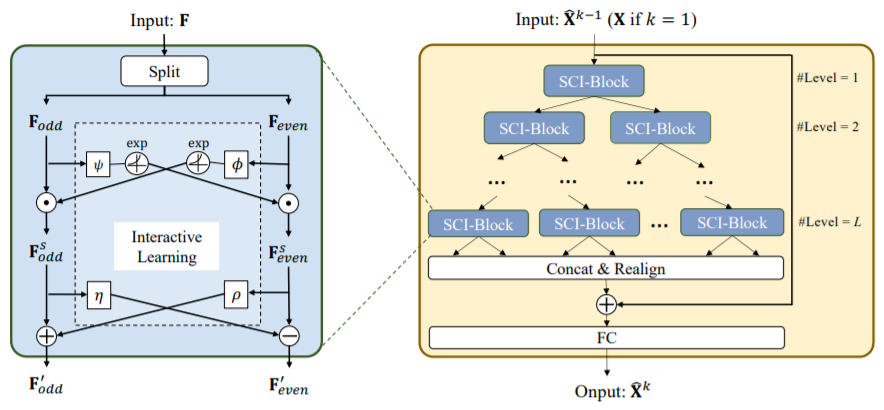
\includegraphics[width=0.48\textwidth]{scinet.png}
    \caption{The architecture of SCINet. On the left is a SCI-Block, and on the right is the SCINet model. We can see that the input of a SCI-Block gets separated and processed interdependently. The imput gets separated multiple times through the model which enables the learning on different resolutions.}
    \label{fig:scinet}
\end{figure}

The SCINet model is hierarchical and is build using SCI-Blocks.
Each SCI-Block splits the data into $F_{odd}$ and $F_{even}$.
It uses different kernels to learn features from each sequence separately.
To compensate for possible information loss while downsampling authors propose interactive learning strategy.
$F_{odd}$ and $F_{even}$ are projected to hidden states with two different 1D convolution functions, $\psi$ and $\phi$.
Then they are transformed using exponential function and perform element-wise product with swapped odd and even sequences, as shown in Equation \ref{eq:scinet_block}.

\begin{equation}
\label{eq:scinet_block}
\begin{split}
    F_{odd}^{s} &= F_{odd} \cdot exp(\psi(F_{even})) \\
    F_{even}^{s} &= F_{even} \cdot exp(\phi(F_{odd}))
\end{split}
\end{equation}

Next, the two scaled feature vectors are again projected to another set of hidden states with two different 1D convolution functions, $\rho$ and $\eta$, and are added or subtracted from $F_{odd}^{s}$ and $F_{even}^{s}$ to get output sequences, $F_{odd}^{'}$ and $F_{even}^{'}$.
The entire process is repeated recursively until we get a tree-like structure.
Authors report that the best results are obtained with fewer than five levels of SCI-Blocks.

The output of the bottom SCI-Blocks is concatenated by reversing the splitting operation and then added to the original sequence.
A fully connected layer is used to output final predictions.
The authors also propose that the output of one SCINet could be fed into another to achieve better prediction accuracy.

\section{Data and Metrices}
\label{chap:data}

In TSF there exist a few popular datasets for models to be tested on.
Most used ones were introduced by Lai et al. in \cite{lai2018lstnet}.
The datasets are electricity, traffic, solar, and exchange.
Their descriptions are available in Table \ref{tab:datasets1}.

\begin{table}[]
    \centering
    \begin{tabular}{r|ccc}
        Dataset & T & D & L \\
        \hline
        Electricity & 26,304 & 321 & 1 hour \\
        Traffic & 17,544 & 862 & 1 hour \\
        Solar & 52,560 & 137 & 10 minutes \\
        Exchange & 7,588 & 8 & 1 day \\
    \end{tabular}
    \caption{Description of datasets. T represents number of timestamps, D the number of variables, and L sample rate of data.}
    \label{tab:datasets1}
\end{table}

The electricity dataset includes the kWh consumption of electricity for 321 clients from years 2011 to 2014.
Data points reflect hourly consumption.
Traffic dataset describes road occupancy rates for 862 roads in San Francisco Bay area, California, USA.
Data was collected for 48 months and has granularity of 1 hour.
Solar energy dataset measures solar production rates for 137 solar power plants in Alabama, USA.
The data was collected every 10 minutes in 2006.
Final common dataset is exchange, which provides daily exchange rates for 8 different currencies from 1990 to 2016.

Another newer dataset was introduced by \cite{zhou2021informer}.
The Electricity Transformer Temperature (ETT) dataset includes one target variable, oil temperature, and has six other variables, denoting power load values.
The data contains two years of values, measured at 15 minute intervals, on two electricity transformers in China.
The dataset has three variations, ETTh1, ETTh2, ETTm1. h1 and h2 versions have sequences with 1 and 2 hour difference respectively. The m1 version has 15 minute sample rate.


The most common metrics used in TSF are mean absolute error (MAE), mean square error (MSE), normalized deviation (ND), root mean square error (RMSE), normalized root mean square error (NRMSE), root relative square error (RSE), and empirical correlation coefficient (CORR). The equations for each metric can be seen in Equation \ref{eq:metrics}.

\begin{equation}
\label{eq:metrics}
\begin{split}
    MAE &= \frac{1}{N}\sum_{i=1}^{N}\lvert y_{i}-f(x_{i})\rvert \\
    MSE &= \frac{1}{N}\sum_{i=1}^{N}(y_{i}-f(x_{i}))^{2} \\
    ND &= \frac{\sum_{i=1}^{N}\lvert y_{i}-f(x_{i})\rvert}{\sum_{i=1}^{N}\lvert y_{i}\rvert} \\
    RMSE &= \sqrt{\frac{1}{N}\sum_{i=1}^{N}(y_{i}-f(x_{i}))^{2}}\\
    NRMSE &= \frac{\sqrt{\frac{1}{N}\sum_{i=1}^{N}(y_{i}-f(x_{i}))^{2}}}{\frac{1}{N}\sum_{i=1}^{N}\lvert y_{i}\rvert} \\
    RSE &= \frac{\sqrt{\sum_{i=1}^{N}(y_{i}-f(x_{i}))^{2}}}{\sqrt{\sum_{i=1}^{N}(y_{i}-\overline{y})^{2}}} \\
    CORR &= \frac{1}{N}\sum_{j=0}^{N}\frac{\sum_{i=0}^{d}(y_{i,j}-\overline{y})(x_{i,j}-\overline{x})}{\sum_{i=0}^{d}(y_{i,j}-\overline{y})^{2}(x_{i,j}-\overline{x})^{2}}
\end{split}
\end{equation}

\section{Results}
\label{chap:results}

In this section we will present the results from evaluating models against the reported metrics.
The evaluated models are TRMF, DeepAR, and SCINet.
ARIMA model is used in the final comparison between models.

Authors of \textbf{TRMF} model performed evaluation on electricity, traffic, and synthetic datasets.
For the synthetic dataset the authors randomly generated matrix $F$ and $x_{i}$ following predefined model with lags.
True values are obtained by $y_{t} = Fx_{t}+\epsilon$, where $\epsilon \sim N(0, 0.01)$.
The electricity and traffic datasets were first standardized.
The authors used ND and NRMSE metrics for forecasting evaluation.
Their results compared to mine are in Table \ref{tab:trmf_exp}.

\begin{table}[htb]
    \centering
    \begin{tabular}{c|cc|cc|cc}
         & \multicolumn{2}{c}{Syntetic} & \multicolumn{2}{c}{Electricity} & \multicolumn{2}{c}{Traffic} \\
         & ND & NRMSE & ND & NRMSE & ND & NRMSE \\
        \hline
        TRMF & 0.373 & 0.487 & 0,255 & 1,397 & 0.187 & 0.423 \\
        Reproduced & 0.330 & 0.443 & 0.562 & 0.941 & 0.57 & 0.618 \\
    \end{tabular}
    \caption{Reproduced results for TRMF model.}
    \label{tab:trmf_exp}
\end{table}

We can see that for syntetic dataset out results were a little bit better than the authors, but that was probably because the data was randomly generated and the authors didn't provide reproducible code.
But we were unable to reproduce the results on the electricity and traffic datasets.
Our experiments achieved higher ND score, but lower NRMSE score for electricity dataset.
On the traffic dataset our evaluations performed worse. Even though the datasets were both standardized, the authors newer explicitly stated their train and test splits.
We used the same prediction horizon and lookback window, but had problems with using the same lags as authors.
We used $[1, 24]$ as lags instead of $[1, \dots, 24, 168, \dots, 191]$ because the combined gradient was too large and hte regularization parameters could not be set low enough.
We performed rolling cross validation on the last two years of data, but we cannot be certain that the authors did the same.
On Figure \ref{fig:trmf_forecast} we can see an example forecast for TRMF model on electricity dataset for a random client.
The model learned the features of the data and made a good prediction, which follows the real trend.

\begin{figure}
    \centering
    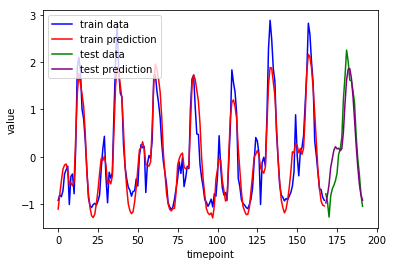
\includegraphics[width=0.48\textwidth]{trmf_forecast.png}
    \caption{Performance of TRMF model on random client in electricity dataset. We can see that the model can capture trends and even forecast with relative percision.}
    \label{fig:trmf_forecast}
\end{figure}

Authors of \textbf{DeepAR} trained and tested their model on five datasets: three public and two private.
The public datasets were parts, traffic, and electricity, and the two private datasets were ec and ec-sub, weekly item sales from Amazon.
We had access only to traffic and electricity datasets, so we tested the DeepAR model on them.
They used the same metrics as authors of TRMF, except they replaced the NRMSE with RMSE.
Their results compared to mine are in Table \ref{tab:deepar_exp}.

\begin{table}[htb]
    \centering
    \begin{tabular}{c|cc|cc}
         & \multicolumn{2}{c}{Electricity} & \multicolumn{2}{c}{Traffic} \\
         & ND & RMSE & ND & RMSE \\
        \hline
        DeepAr & 0.07 & 1.00 & 0,17 & 0,42 \\
        Reproduced & 0.369 & 0.445 & 0.669 & 0.988 \\
    \end{tabular}
    \caption{Reproduced results for DeepAR model.}
    \label{tab:deepar_exp}
\end{table}

The reproduced results for electricity dataset were a bit unusual.
Reproduced ND score was higher than the one reported by the authors, but the reproduced RMSE score was much lower.
The results for traffic dataset are worse as well, but at least both metrics are worse by a factor.
Higher metric values may be due to training time.
The authors state that training on electricity and traffic datasets took 7 and 3 hours respectively, while ours took around 10 minutes.
We used the same network structure, but limited training to 200 epochs with early stopping if results have not improved for 20 epochs.
The authors did not mention such training parameters.

When looking deeper into the article we noticed that they used slightly different RMSE formula, and their naming of metrics is not consistent.
In the text they mention normalized RMSE or NRMSE and present a modified NRMSE formula, but they use RMSE when presenting results.
If we calculate NRMSE for each dataset, we get much lower values than the ones presented by authors.

The authors of \textbf{SCINet} model tested their model on all previously described datasets, but included only ETT results in their published paper.
Unpublished version of the paper includes results for electricity, exchange, traffic, and solar datasets, which we tried to replicate.
For their purposes authors chose metrics RSE and CORR.
In Table \ref{tab:scinet_exp} we can see reproduced results for electricity, solar, and exchange datasets.
We did not reproduce traffic dataset due to memory constraints.

\begin{table}[thb]
    \centering
    \begin{tabular}{c|cc|cc|cc}
         & \multicolumn{2}{c}{Electricity} & \multicolumn{2}{c}{Solar} & \multicolumn{2}{c}{Exchange} \\
         & RSE & CORR & RSE & CORR & RSE & CORR \\
        \hline
        SCINet & 0.0957 & 0.9276 & 0.4032 & 0.9413 & 0.0426 & 0.9591 \\
        Reproduced & 0.1041 & 0.9218 & 0.4079 & 0.9112 & 0.0445 & 0.9273 \\
    \end{tabular}
    \caption{Reproduced results for SCINet model.}
    \label{tab:scinet_exp}
\end{table}

We can see that we were able to reproduce all of their results with a reasonable margin of error.
The reproduced scores are a little bit worse than the ones authors presented, but are close.
Such results are expected, as authors trained their model for 100 epochs while we trained it only for 30.

All of the previously tested models were also trained on ETT dataset to compare them directly, since different authors used different metrics.
We used the ETTh1 dataset, which has granularity of 1 hour.
The authors of SCINet were kind enough to test DeepAR and ARIMA on ETTh1 dataset, so we can compare our findings to theirs.
For baseline we use the ARIMA model.
The DeepAR and TRMF models have the same architecture as the authors used for their testing.
The models were tested with univariate forecasting, except for TRMF, which requires multiple time series sequences.
The TRMF model was evalueated only on the one sequence other models were tested on.
The reproduced results can be seen on Table \ref{tab:ett_exp}.
The results the authors of SCINet provided are in Table \ref{tab:ett_scinet}.

\begin{table}[thb]
    \centering
    \begin{tabular}{cc|ccccc}
         & Horizon & 24 & 48 & 168 & 336 & 720 \\
        \hline
        \multirow{2}{*}{ARIMA} & MAE & 0.324 & 0.248 & 0.240 & \textbf{0.201} & \textbf{0.303} \\
         & MSE & 0.155 & 0.098 & 0.087 & \textbf{0.065} & \textbf{0.143} \\
        \hline
        \multirow{2}{*}{TRMF} & MAE & 1.043 & 0.937 & 0.900 & 0.899 & 1.080 \\
         & MSE & 1.141 & 0.940 & 0.879 & 0.860 & 1.254 \\
        \hline
        \multirow{2}{*}{DeepAR} & MAE & 0.146 & 0.195 & 0.238 & 0.246 & 0,343 \\
         & MSE & 0.036 & 0.062 & 0.088 & 0.092 & 0.168 \\
        \hline
        \multirow{2}{*}{SCINet} & MAE & \textbf{0.134} & \textbf{0.170} & \textbf{0.222} & 0.253 & 0.348 \\
         & MSE & \textbf{0.031} & \textbf{0.050} & \textbf{0.082} & 0.102 & 0.181 \\
    \end{tabular}
    \caption{Results on ETTh1 dataset. The best results are in \textbf{bold}.}
    \label{tab:ett_exp}
\end{table}

\begin{table}[thb]
    \centering
    \begin{tabular}{cc|ccccc}
         & Horizon & 24 & 48 & 168 & 336 & 720 \\
        \hline
        \multirow{2}{*}{ARIMA} & MAE & 0.284 & 0.424 & 0.504 & 0.593 & 0.766 \\
         & MSE & 0.108 & 0.175 & 0.396 & 0.468 & 0.659 \\
        \hline
        \multirow{2}{*}{DeepAR} & MAE & 0.280 & 0.327 & 0.422 & 0.552 & 0.707 \\
         & MSE & 0.107 & 0.162 & 0.239 & 0.445 & 0.658 \\
        \hline
        \multirow{2}{*}{SCINet} & MAE & 0.132 & 0.173 & 0.222 & 0.242 & 0.343 \\
         & MSE & 0.031 & 0.051 & 0.081 & 0.094 & 0.176 \\
    \end{tabular}
    \caption{Results on ETTh1 dataset from the authors of SCINet.}
    \label{tab:ett_scinet}
\end{table}

\begin{figure}[htb]
    \centering
    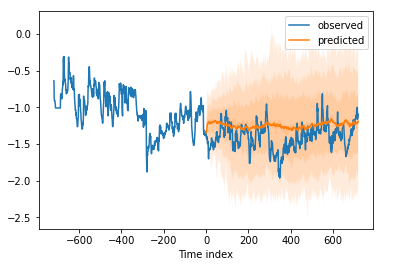
\includegraphics[width=0.48\textwidth]{deepar_eth.png}
    \caption{Performance of DeepAR model on OT variable in ETTh1 dataset. Since DeepAR is a probabilistic mode, we can see how the prediction distribution changes through time, but does not get larger, meaning the model is consistent with future predictions.}
    \label{fig:deepar_forecast}
\end{figure}

If we first take a look at SCINet's authors results at Table \ref{tab:ett_scinet} we can see that SCINet is the clear winner, with DeepAR taking second place and ARIMA third.
Since ARIMA is the most simple of the three models, the results are expected.
We can also see that the MAE and MSE scores are higher for longer forecasting windows.

If we take a look at our results at Table \ref{tab:ett_exp} the scores are different.
Not much has changed for SCINet compared to their reported scores, but the other models could not be replicated.
DeepAR model performed twice as better as authors of SCINet reported it to be.
This is strange since our MAE metric for DeepAR is constantly around half the reported values of SCINet paper.
The forecast of the DeepAR model for a horizon of 720 can be seen of Figure \ref{fig:deepar_forecast}, where we can see that the model has low variance.
The ARIMA model has the highest difference from reported values and has scored the best for longer horizons, which is unexpected.
It was also unexpected that the results do not change much when we increase the forecasting horizon.
Upon closer inspection we realised that longer forecasts for ARIMA tend to converge to one number, which in our case was around the average of the testing sequence and thus produced nearly constant MAE and MSE scores regardless of forecasting horizon length.
The TRMF model is the only one which was multivariate, but we focused only on target variable.
The model produces consistent scores with MAE and MSE metrics like ARIMA, and upon inspection we saw that it could not replicate the input sequence like it did when forecasting on electricity dataset.
It also had the same problem as ARIMA, where it forecasted a constant value, which happened to be around the average of the testing sequence.

At the end the best model on ETTh1 dataset is SCINet, DeepAR placed second, ARIMA third, and TRMF fourth. DeepAR took second place because it performed much better for shorter horizons than ARIMA.
Since SCINet is currently state-of-the-art its dominance was expected.

\section{Conclusion}

The aim of this report was to present the state of TSF and currently used models. We presented in detail matrix factorization, transformer, and other deep models. We presented the most popular datasets and metrics used for TSF.
We tried to replicate the results from three different papers and were largely unsuccessful. When comparing the models on the same dataset the results were expected, and we confirmed that SCINet is current state-of-the-art model for TSF.

%\section*{Acknowledgment}

%The authors would like to thank...

\printbibliography[heading=bibintoc,title={References}]

\end{document}


